\chapter{Materiais e Métodos}
Neste capítulo são apresentados os materiais necessários para o desenvolvimento deste projeto bem como todos os procedimentos seguidos para levar os resultados apresentados.

\section{Materiais}
    No presente trabalho foram utilizados diversos materiais e ferramentas computacionais, sendo que os principais compreendem:
	\begin{itemize}
		\item Placa de desenvolvimento com microcontrolador STM32F103C8T6;
		\item Módulo \textit{display} LCD 16x2 HD44780;
		\item Luva de sensores construída manualmente;
		\item Sensor inercial MPU-6050;
		\item Circuito condicionador de sinal;
		\item IDE de programação para família de microcontroladores STM32(Atollic);
		\item Depurador/programador ST-Link/V2;
		\item Interpretador da linguagem Python.
	\end{itemize}

	
	\subsection{Placa de desenvolvimento com microcontrolador STM32F103C8T6}
	
		A referida placa de desenvolvimento, ilustrada na Figura \ref{fig:micro}, possui um microcontrolador ARM-Cortex M3  de 32 bits com 20kB de memória SRAM e e 64 kB de memória flash. Ainda contém2 conversores A/D (Analógico para digital) de 12 bits, 3 temporizadores de propósito geral e até 37 portas de entrada e saída tolerantes a 5V \cite{STM32F103}.
        
        \begin{figure}[H]
            \centering
            \caption{Microcontrolador STM32F103C8T6}
            \label{fig:micro}
            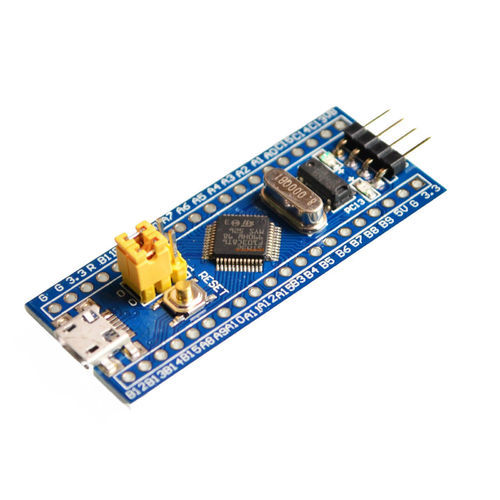
\includegraphics[scale=0.5]{imagens/micro.jpg}
            \caption*{Fonte: \citeonline{indiamart}.}

        \end{figure}
        
	\subsection{Módulo \textit{display} LCD 16x2 HD44780}
	
	    O módulo HD44780 \textit{display} de matrizes de pontos feito é com cristal liquido que pode reproduzir alfanuméricos, caracteres japoneses e símbolos customizados. Pode ser configurado para operar com transferência de 8 bits ou 4 bits. Todas as operações efetuadas para manipulação do \textit{display} são feitas na memória do controlador interno, sendo fornecido um driver transforma as informações escritas na memória para a tela de cristal liquido. O referido \textit{display} tem compatibilidade de pinagem com outros lcds de 16x2 para ser facilmente trocado caso haja necessidade. A baixa tensão de operação (2.7V até 5.5V) permite que o \textit{display} seja utilizado em sistemas ligados a bateria \cite{hitachi}.
    	Na Figura \ref{fig:hd44780} está o \textit{display} HD44780.
    	
    	\begin{figure}[H]
    	    \centering
     	    \caption{\textit{Display} LCD 16x2 de cristal líquido HD44780}
      	    \label{fig:hd44780}
    	    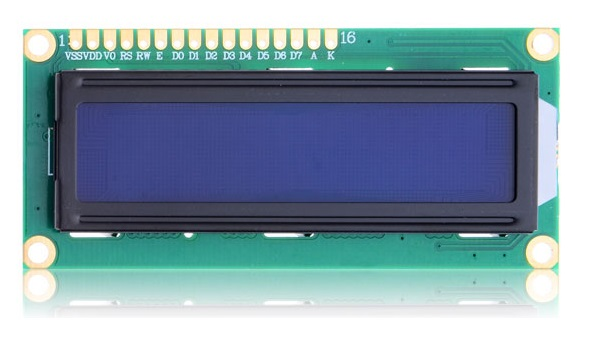
\includegraphics[scale=0.5]{imagens/hd44780.jpg}
    	    \caption*{Fonte: \citeonline{filipeflopHD}.}

    	\end{figure}
	
	\subsection{Sensor inercial MPU-6050}
    	O dispositivo MPU6050 é um sensor inercial de 6 eixos integrados que combina 3 eixos de giroscópio e 3 eixos de acelerômetro, e conta com um processador digital de movimentos, isso tudo em  um encapsulamento de 4x4x0,9 mm. Utilizado com comunicação I2C, o sensor aceita entradas de um compasso externo de 3 eixos para retornar uma fusão de coordenadas de movimento de 9 eixos \cite{mpu6050}.
        
        O dispositivo MPU6050 também possui internamente 3 conversores A/D (Analógico para digital) de 16 bits para giroscópio e 3 conversores A/D para acelerômetro afim de converter as entradas analógicas dos sensores. A escala de operação do acelerômetro é programável e pode ser escolhida entre  ±2g, ±4g, ±8g, e ±16g. O mesmo ocorre para o giroscópio, que tem as escalas de operação de ±250, ±500, ±1000, e ±2000°/sec \cite{mpu6050}. A Figura \ref{fig:mpu6050} ilustra a placa com o sensor MPU-6050 utilizada no presente projeto.

        \begin{figure}[H]
        	\vspace{4mm}
            \centering
            \caption{Sensor inercial MPU6050}
            \label{fig:mpu6050}
            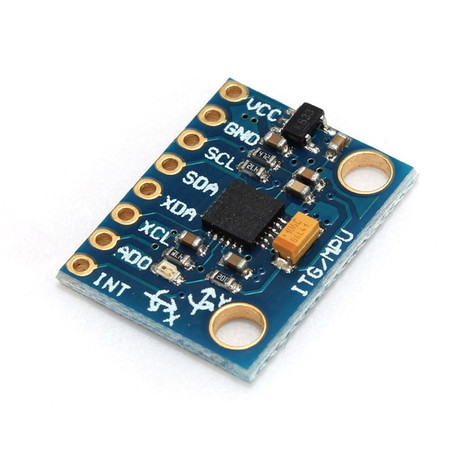
\includegraphics[scale=0.3]{imagens/mpu6050.jpg}
            \caption*{Fonte: \citeonline{filipeflopHD}.}

        \end{figure}
        
        
        \subsection{Conjunto de luva e circuito de condicionamento de sinais}
        A luva sensora, demonstrada na Figura \ref{fig:luva}, contém as bobinas sensoras e geradoras, todas ligadas ao um conector. 
\begin{figure}[H]
   	\vspace{4mm}
   	\centering
   	\caption{Luva sensora desenvolvida por \citeonline{RUANI}}
   	\label{fig:luva}
   	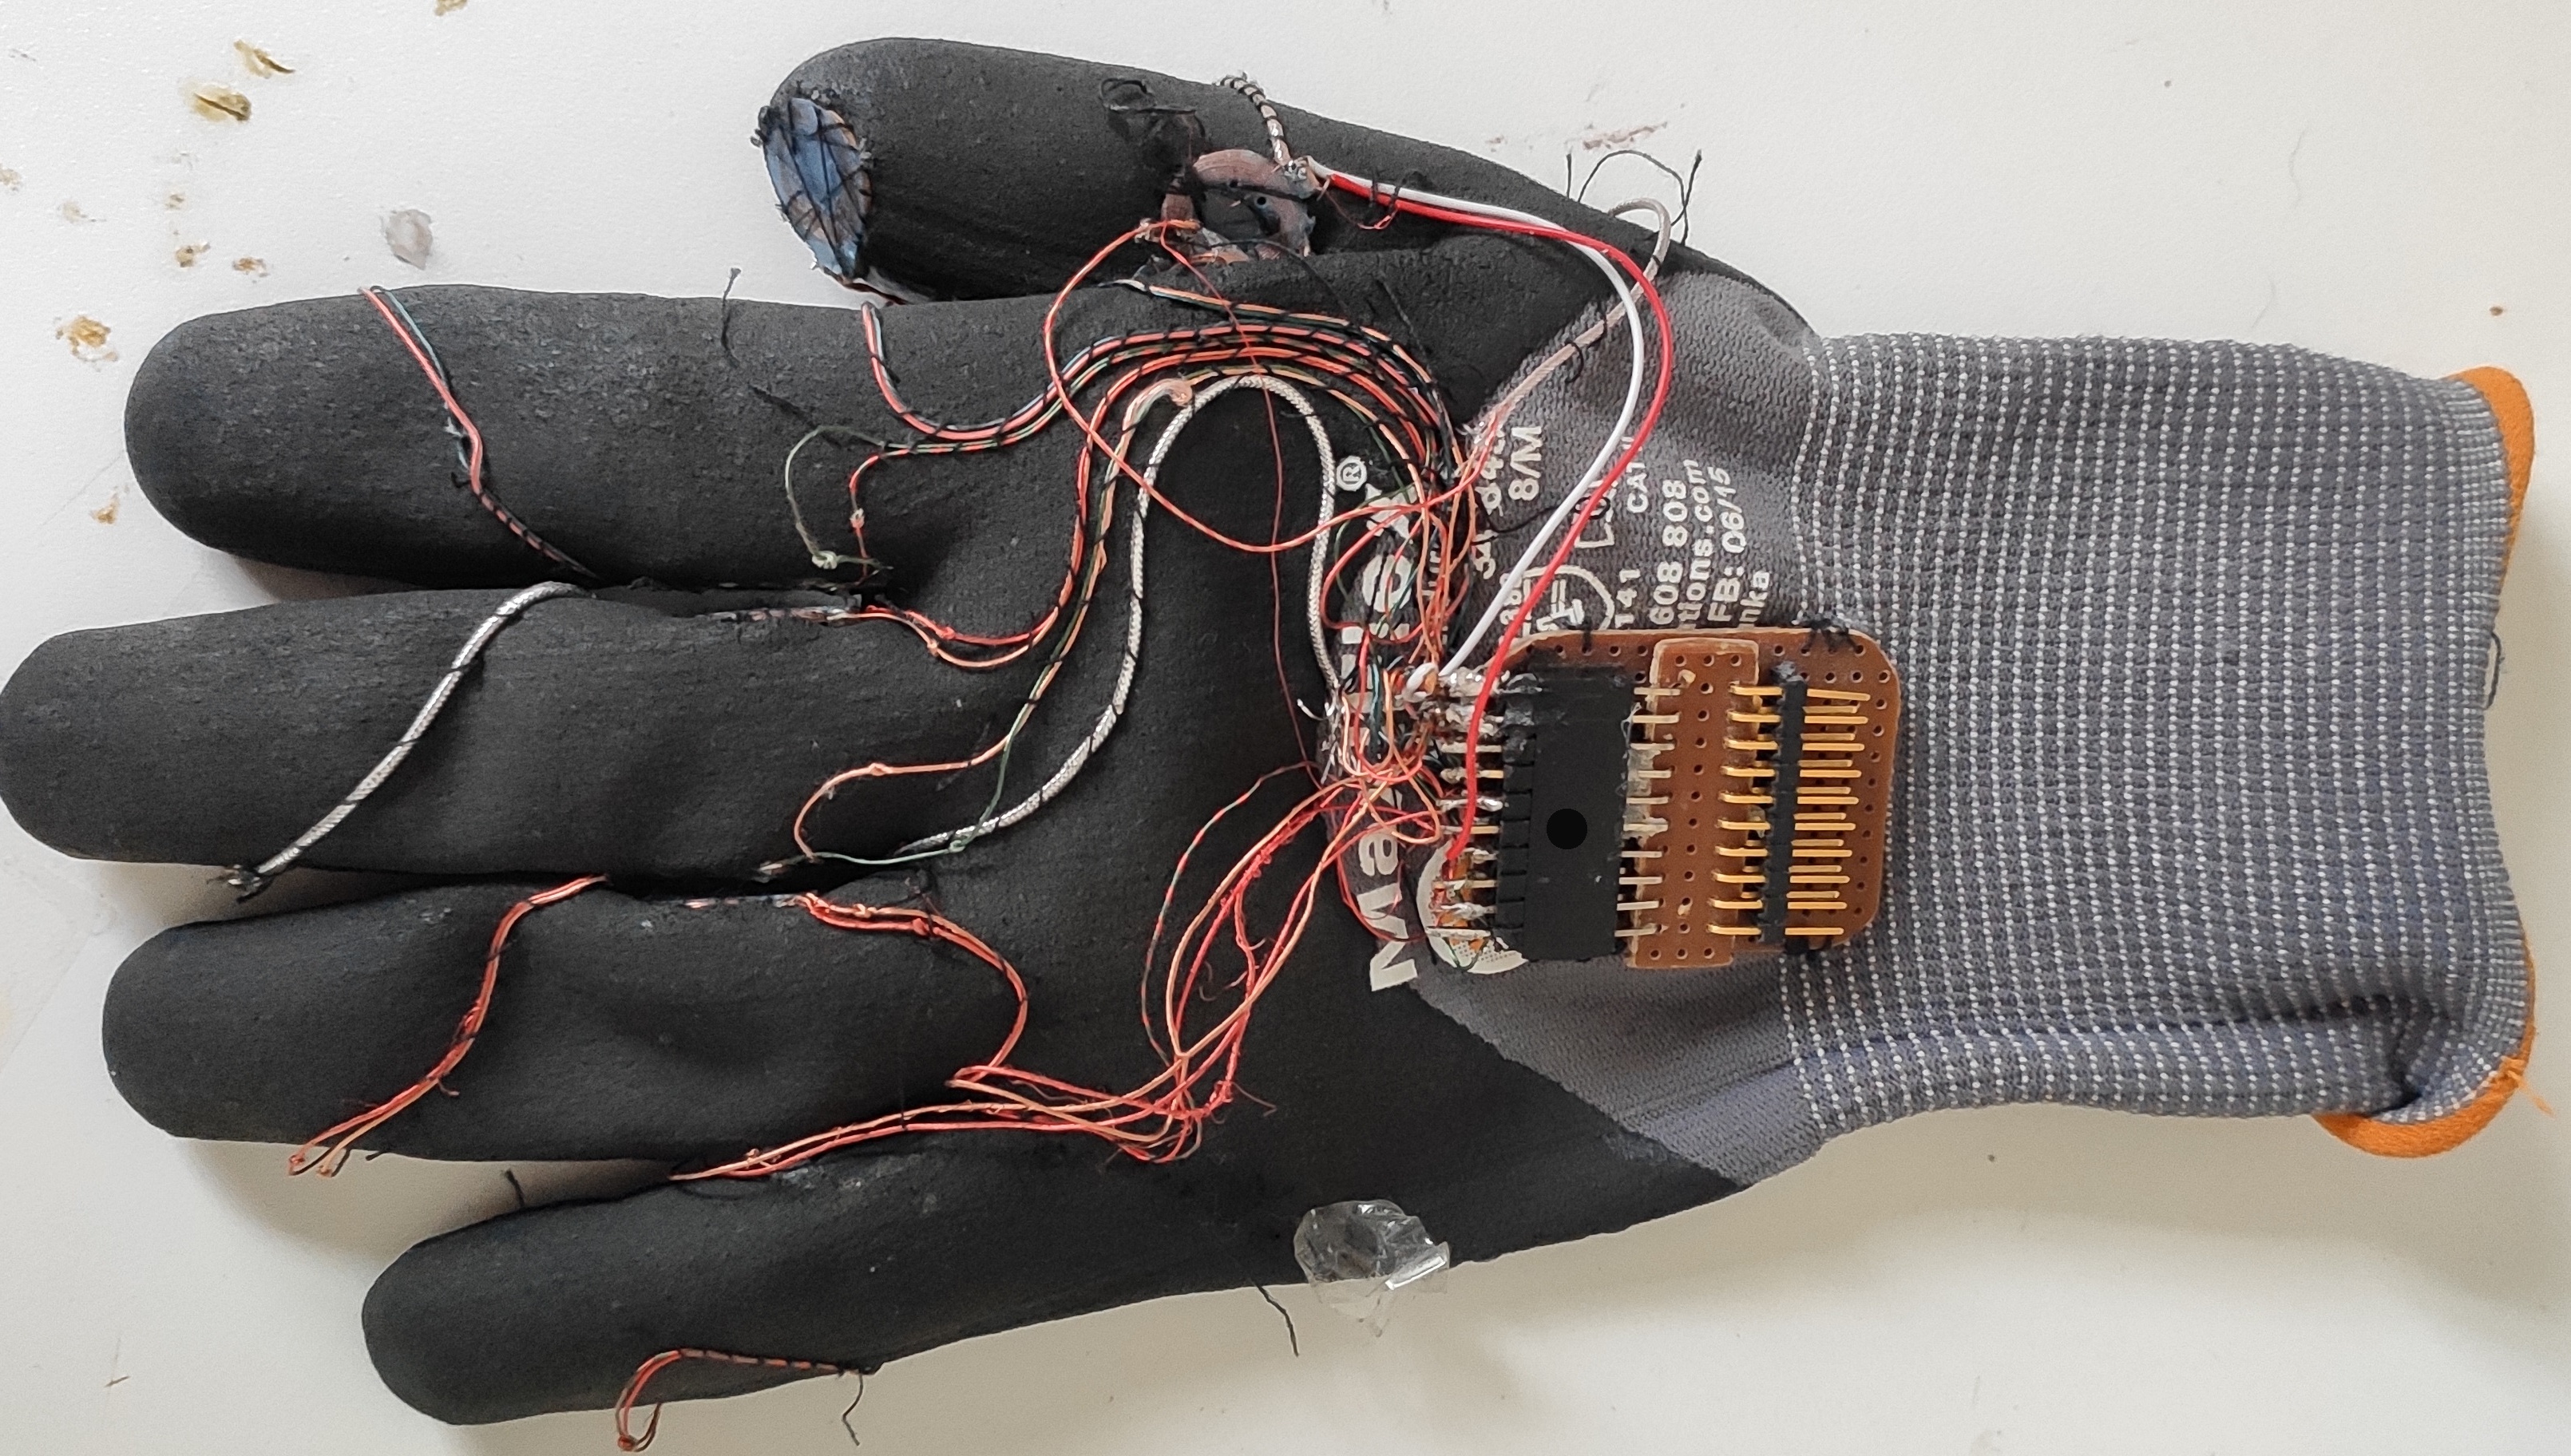
\includegraphics[scale=0.10]{imagens/luva_so.jpg}
   	\caption*{Fonte: Autoria própria.}
\end{figure}

A luva e conectada a placa de processamento de sinais das bobinas da Figura \ref{fig:placa1}. O funcionamento desta placa foi demonstrado na sessão \ref{sec:placa}. 

\begin{figure}[H]
   	\vspace{4mm}
   	\centering
   	\caption{Placa para recepção e processamento dos sinais vindos do sensor indutivo}
   	\label{fig:placa_in1}
   	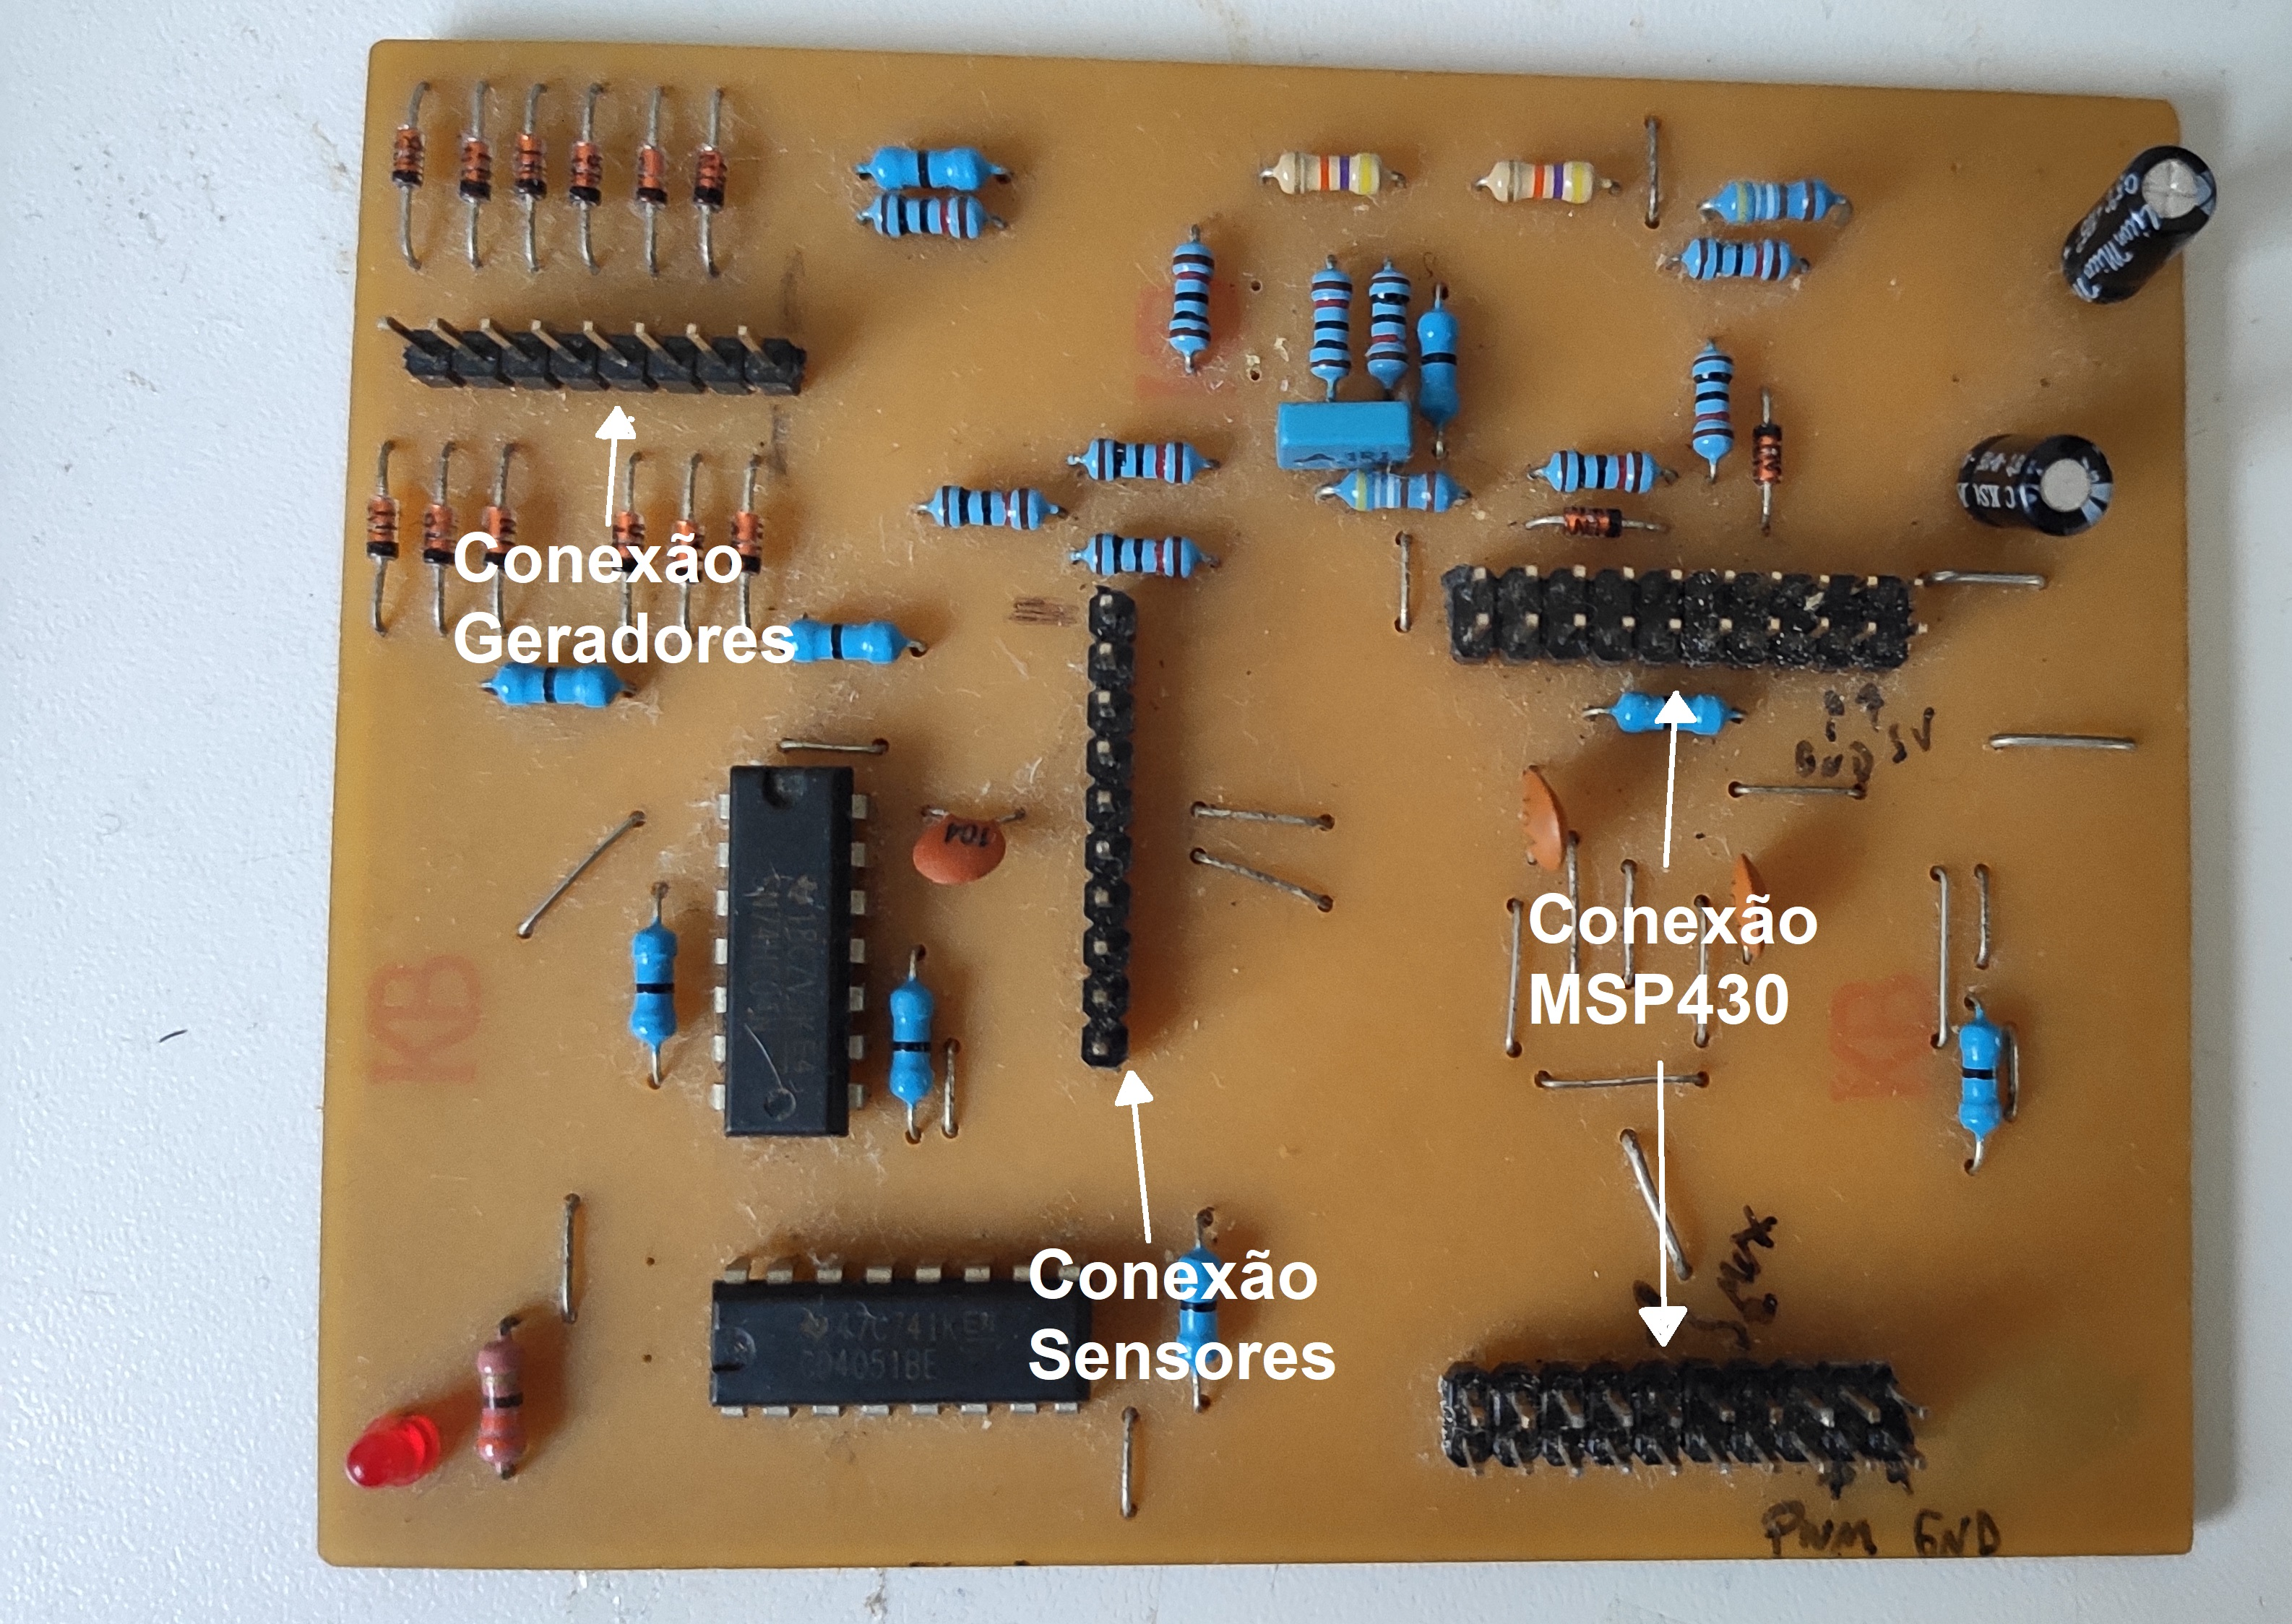
\includegraphics[scale=0.10]{imagens/placa_ruani.jpg}
   	\caption*{Fonte: Autoria própria.}
\end{figure}
	
A conexão é para o microcontrolador MSP430F5529, onde será encaixada uma placa de adaptação para o microcontrolador STM32F103C8T6.        